\newpage
\subsection{Turning a Card around (Invert)}

The next SDM \emph{inverts} a card by swapping its back and face values. This therefore ``turns the card around'' in the learning box, which makes sense when
learning, for example, a new language. You're no longer an SDM beginner so try to model the SDM depicted in Fig.~\ref{fig:sdm_invert}.

\begin{figure}[htbp]
\begin{center}
  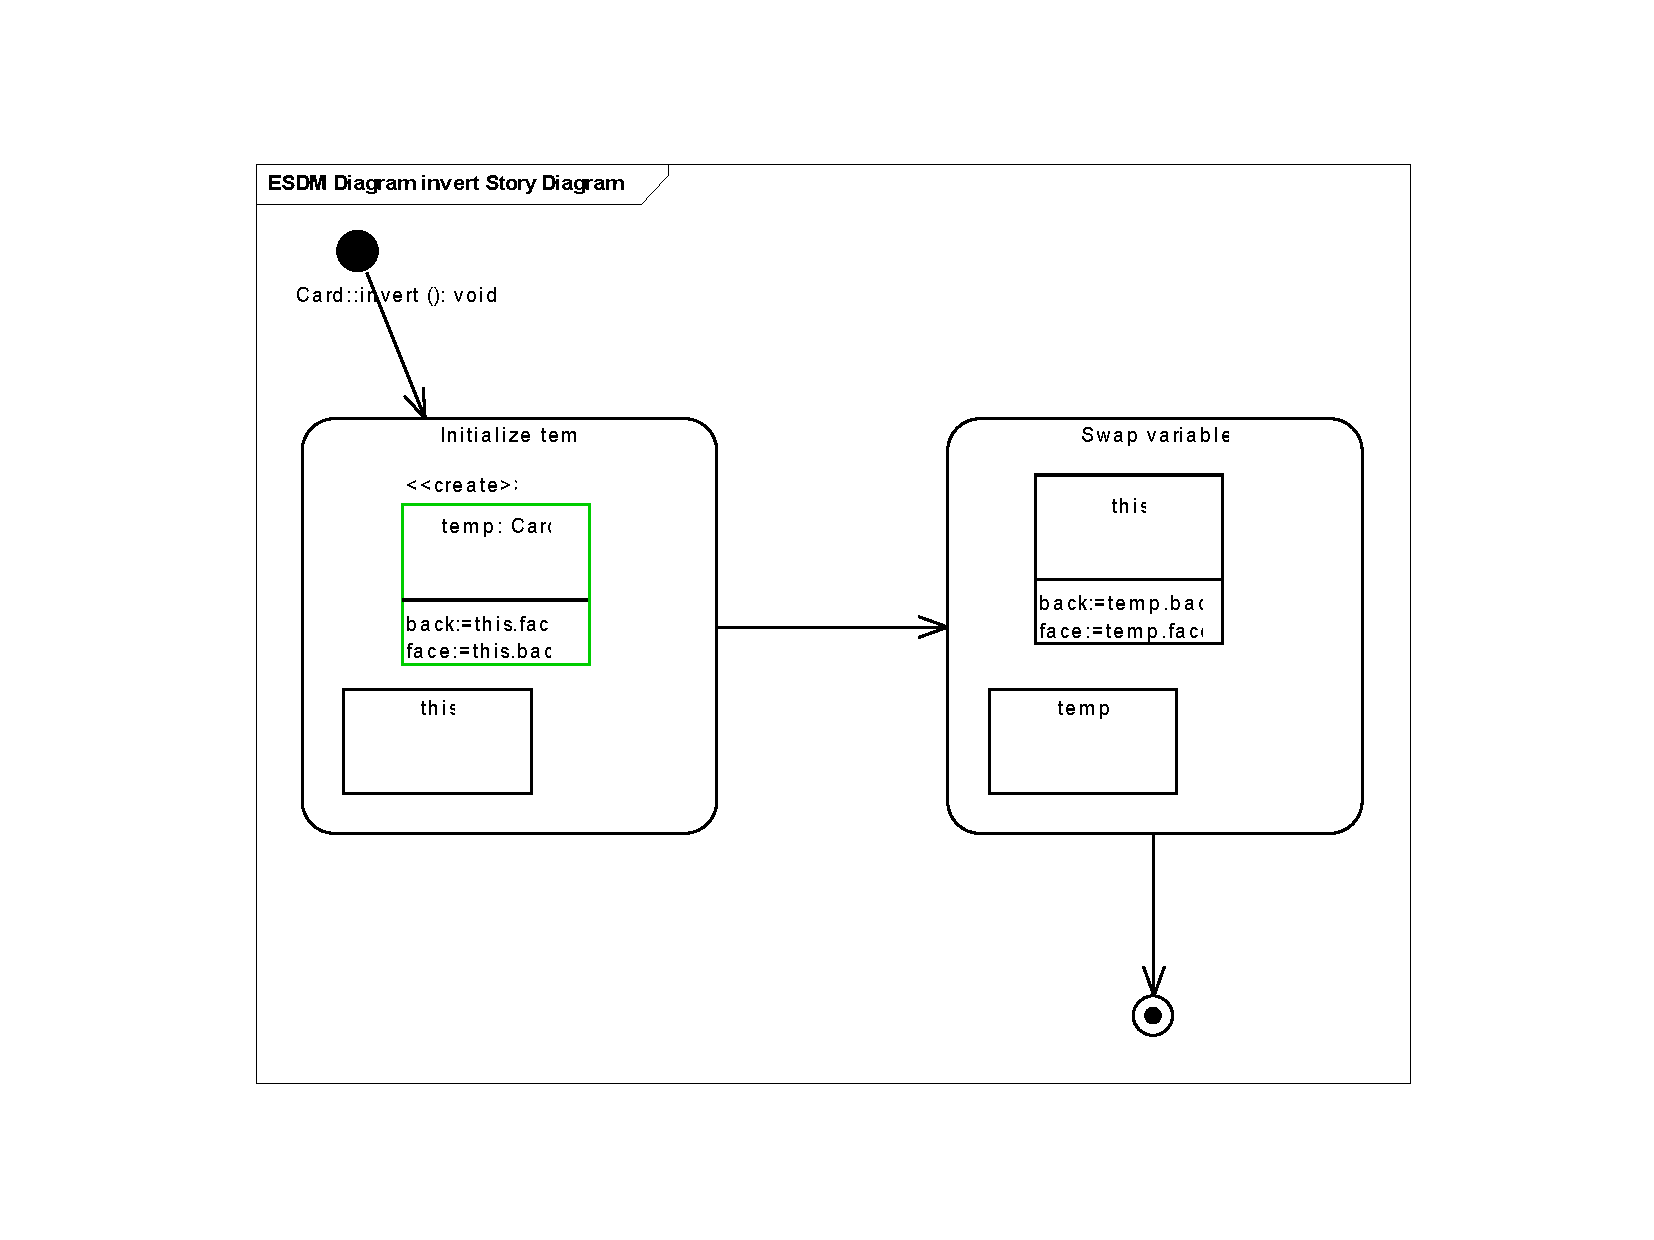
\includegraphics[width=0.6\textwidth]{sdm54}
  \caption{Swap back and face of the card.}  
  \label{fig:sdm_invert}
\end{center}
\end{figure}

Something new here is that we use \emph{assignments} to set the attributes of\note{Assignments} \texttt{temp} in \texttt{Initialize temp} and to swap the
attributes of \texttt{this} in \texttt{Swap variables}. An assignment is an attribute constraint with \texttt{:=} as operation.  Although it might be slightly
confusing to refer to an assignment as a constraint, if you think a while about it \emph{everything} can be viewed as a constraint that can be fulfilled via
different strategies. In this case, an assignment is fulfilled not by searching \note{Assertion} for a match, as in the case of an assertion (\texttt{==, >, <,
\ldots}), but by \emph{performing} the assignment. Similarly, non-context elements (set to create or destroy) can be viewed as structural constraints that are
fulfilled by creating or destroying the corresponding element.  A constraint is therefore a unifying concept similar to ``everything is an object'' from OO and
``everything is a model'' from metamodelling and has the usual advantages.  If \note{Unification} you're interested in why unification is considered cool check
out \cite{BEZ05}.

A last point before we move on to the next SDM.  Did you notice that \texttt{temp} is bound in the story pattern of \texttt{Swap variables}?  This is a new case
for bound variables that we haven't treated yet. Until now we have seen object variables that can be (1) bound to an argument of the method that is set when the
method is invoked, or (2) bound to the current object \texttt{this} whose method is invoked. In both cases, the object to be matched is completely determined by
the context of the method and does not need to be determined by the pattern matcher.

Setting \texttt{temp} as bound in \texttt{Swap variables} is a third case in which an object variable is bound to the value already determined in a
\emph{previous activity node}. This means that in our case, the object variable \texttt{temp} in \texttt{Swap variables} is to be bound to the value determined
for the unbound object variable \texttt{temp} in \texttt{Initialize temp}. This way, you can always refer to previous matches for object variables in the
preceding control flow. Please note that the reference or mapping is again implicit via the same \emph{name} of the object variable.
As in the case of arguments of the method, the editor provides rudimentary support via a drop-down menu which can be used to choose the name of an object
variable and avoid possible mistakes when typing by hand.
